%%%%%%%%%%%%%%%%%%%%%%%%%%%%%%%%%%%%%%%%%%%%%%%%%%%%%%%%%%%%%%%%%%%%%%%%%%%%%%%%
%%%%%%%%%%%%%%%%%%%%%%%%%%%%%%%%%%%%%%%%%%%%%%%%%%%%%%%%%%%%%%%%%%%%%%%%%%%%%%%%
%%% Template for AIMS Rwanda Assignments         %%%              %%%
%%% Author:   AIMS Rwanda tutors                             %%%   ###        %%%
%%% Email: tutors2017-18@aims.ac.rw                               %%%   ###        %%%
%%% Copyright: This template was designed to be used for    %%% #######      %%%
%%% the assignments at AIMS Rwanda during the academic year %%%   ###        %%%
%%% 2017-2018.                                              %%%   #########  %%%
%%% You are free to alter any part of this document for     %%%   ###   ###  %%%
%%% yourself and for distribution.                          %%%   ###   ###  %%%
%%%                                                         %%%              %%%
%%%%%%%%%%%%%%%%%%%%%%%%%%%%%%%%%%%%%%%%%%%%%%%%%%%%%%%%%%%%%%%%%%%%%%%%%%%%%%%%
%%%%%%%%%%%%%%%%%%%%%%%%%%%%%%%%%%%%%%%%%%%%%%%%%%%%%%%%%%%%%%%%%%%%%%%%%%%%%%%%


%%%%%% Ensure that you do not write the questions before each of the solutions because it is not necessary. %%%%%% 

\documentclass[12pt,a4paper]{article}

%%%%%%%%%%%%%%%%%%%%%%%%% packages %%%%%%%%%%%%%%%%%%%%%%%%
\usepackage{amsmath}
\usepackage{amssymb}
\usepackage{amsthm}
\usepackage{amsfonts}
\usepackage{graphicx}
\usepackage[all]{xy}
\usepackage{tikz}
\usepackage{verbatim}
\usepackage{float}
\usepackage[left=2cm,right=2cm,top=3cm,bottom=2.5cm]{geometry}
\usepackage{hyperref}
\usepackage{caption}
\usepackage{subcaption}
\usepackage{psfrag}
\usepackage{mathrsfs}
\usepackage{actuarialangle}
\usepackage[T1]{fontenc}
\usepackage{float}
%%%%%%%%%%%%%%%%%%%%% students data %%%%%%%%%%%%%%%%%%%%%%%%
\newcommand{\student}{Yusuf Brima}
\newcommand{\course}{Fluid Mechanics}
\newcommand{\assignment}{1}

%%%%%%%%%%%%%%%%%%% using theorem style %%%%%%%%%%%%%%%%%%%%
\newtheorem{thm}{Theorem}
\newtheorem{lem}[thm]{Lemma}
\newtheorem{defn}[thm]{Definition}
\newtheorem{exa}[thm]{Example}
\newtheorem{rem}[thm]{Remark}
\newtheorem{coro}[thm]{Corollary}
\newtheorem{quest}{Question}[section]

%%%%%%%%%%%%%%  Shortcut for usual set of numbers  %%%%%%%%%%%

\newcommand{\N}{\mathbb{N}}
\newcommand{\Z}{\mathbb{Z}}
\newcommand{\Q}{\mathbb{Q}}
\newcommand{\R}{\mathbb{R}}
\newcommand{\C}{\mathbb{C}}

%%%%%%%%%%%%%%%%%%%%%%%%%%%%%%%%%%%%%%%%%%%%%%%%%%%%%%%555
\begin{document}

%%%%%%%%%%%%%%%%%%%%%%% title page %%%%%%%%%%%%%%%%%%%%%%%%%%
\thispagestyle{empty}
%\begin{figure}
%    \centering
%    \includegraphics[width=\textwidth]{aims_rwanda.jpg}
%\end{figure}
\begin{center}
\textbf{AFRICAN INSTITUTE FOR MATHEMATICAL SCIENCES \\[0.5cm]
(AIMS RWANDA, KIGALI)}
\vspace{1.0cm}
\end{center}

%%%%%%%%%%%%%%%%%%%%% assignment information %%%%%%%%%%%%%%%%
\noindent
\rule{17cm}{0.2cm}\\[0.3cm]
Name: \student \hfill Assignment Number: \assignment\\[0.1cm]
Course: \course \hfill Date: \today\\
\rule{17cm}{0.05cm}
\vspace{1.0cm}
\section*{Exercise 1}
Given the $2^{\text{nd}}$ order linear ODE
\begin{equation}
		\frac{d^2z}{dt^2}   + 3 \frac{dz}{dt} + 3z  = 0
		\label{eq:1}
\end{equation}
\begin{enumerate}
			\item[(a)] The general solution.\\
				We let 
					\begin{equation}
							z(t) =  e^{rt} 
							\label{eq:2}
					\end{equation}
					\begin{equation}
							\therefore \frac{dz}{dt}  =  re^{rt} 
							\label{eq:3}
					\end{equation}
					\begin{equation}
						\text{and } 	\frac{d^2z}{dt^2} =  r^2 e^{rt}
						\label{eq:4}
					\end{equation}
				we substitute \eqref{eq:2} ,  \eqref{eq:3} and \eqref{eq:4}  into \eqref{eq:1} which results in:
						\begin{align*}
								r^2e^{rt} + 3re^{rt} + 3e^{rt} &= 0\\
								(r^2 + 3r + 3)e^{rt} &= 0\\
								\therefore r^2 + 3r + 3 &=  0\\
						\end{align*}
						$a  = 1,  b  =  3, c =  3$
						\begin{align*}
								r &=  \frac{  -b \pm \sqrt{ b^2 - 4ac}  }{ 2a}\\
								&= \frac{-3  \pm  \sqrt{3^3 -  4(1\times 3)  } }{(2 \times 1)}\\
								&= \frac{ -3 \pm \sqrt{ -3} }{ (2)}\\
								&=   \frac{ -3 +  \sqrt{ 3i} }{ (2)} ,  \frac{ -3  - \sqrt{ 3i} }{ (2)}
						\end{align*}
						\begin{align*}
								r_1 &=  \alpha = \frac{-3}{2},  \beta =  \frac{\sqrt{3}}{2}\\
								r_2 &=  \alpha = \frac{-3}{2},  \beta =  \frac{\sqrt{3}}{2}\\
							z(t) &= e^{\alpha t}  \left(   A\cos(\beta t)  + B \sin(\beta t)  \right)\\
							z(t) &=  e^{  \frac{-3}{2}  t } \left(  A\cos \left( \frac{\sqrt{3}}{2} t \right)  + B \sin \left( \frac{\sqrt{3}}{2} t\right)   \right)
						\end{align*}
					The general solution is thus:		
					\begin{equation}
								z(t) =  e^{  \frac{-3}{2}  t } \left(  A\cos \left( \frac{\sqrt{3}}{2} t \right)  + B \sin \left( \frac{\sqrt{3}}{2} t\right)   \right)
								\label{eq:1a}
					\end{equation}										
			\item[(b)]  The particular solutions under the initial conditions, 
			\begin{align*}
			     z(0) &= 1 \\
				\frac{dz} {dt} (0) &=0
			\end{align*}
			From \eqref{eq:1a}
			\begin{align*}
					z(0 &=  e^0 \left(  A\cos(0) + B\sin(0) \right) =1\\
					    \therefore A   &= 1
			\end{align*}
			Also from  \eqref{eq:1a}
			\begin{align*}
					\frac{dz}{dt}(0) &=  \frac{-3}{2} A + frac{ -3  - \sqrt{ 3i} }{ (2)} B  =  0\\
			\end{align*}
			\begin{align*}
					1  &=  A\\
					 0 &= \frac{-3}{2} A +  \frac{ \sqrt{3} }{2}B \\
					 B &= \sqrt{3}
			\end{align*}
			The particular solution is thus:
			\begin{equation}
					z(t) = e^{\frac{-3}{2} t} \left(   \cos\left(\frac{3}{2} t \right)  + \sqrt{3} \sin\left(\frac{3}{2} t \right)   \right)
					\label{eq:1part}
			\end{equation}
			\pagebreak
		\item[(c)] A plot of the trajectories.
							\begin{figure}[!h]
									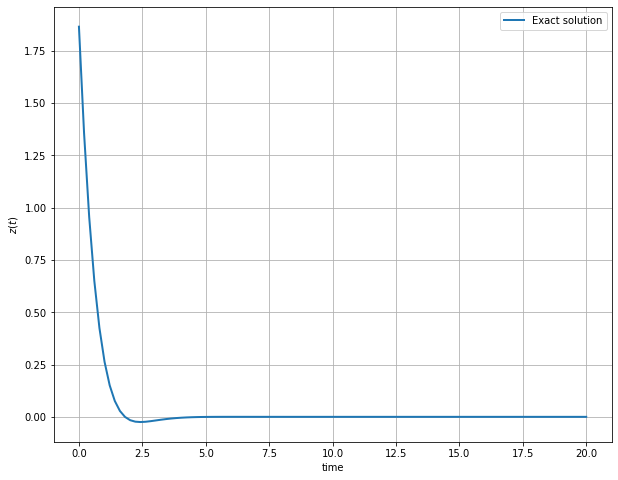
\includegraphics[width=430pt,  height=215pt]{./graphics/q001_c.png}
										\caption{A plot of the particular solution of the  $2^{\text{nd}}$ order linear ODE,}
										\label{fig:q1}
								\end{figure}
\end{enumerate} 
\section*{Exercise 2}
	The motion of a mass around an equilibrium position in a system of
spring-mass-damper system can be described by the following 2nd order linear
ODE
	\begin{equation}
			m\frac{d^t}{dt^2}   + \gamma \frac{dz}{dt} + kz = 0 \quad \text{where } m > 0 , \gamma > 0, k > 0
		\label{eq:2a}
	\end{equation}
		Let $z(t)  =  e^{rt}  ,  \frac{dz}{dt}  =  re^{rt},  \frac{d^z}{dt^2}  =  r^2e^{rt}$\\
		Substituting the above expressions in \eqref{eq:2a}, one gets 
		\begin{align*}
					mr^2e^{rt} + \gamma re^{rt} + ke^{rt} &=  0\\
					\text{Discriminant } D &=  \gamma^2 -  4mk\\		
		\end{align*}
	The resulting the characteristic equation is thus:
		\begin{align*}
					mr^2 + \gamma r + k &=  0\\
					\text{ with the discriminant } D &=  \gamma^2 -  4mk\\		
		\end{align*}
		we observe the 3 cases:
		\begin{enumerate}
			\item[(1)] $D < 0$\ (This will be an \textbf{under-damped system}  $\gamma$  is small relative to $m $and $ k$)\\
					   We have
characteristic roots
					\begin{align*}
							& r_1 =  \frac{ - \gamma }{ 2m}  + \frac{  \sqrt{  \gamma^2  -4mk }}{  2m}  , \quad r_2  = \frac{ - \gamma }{ 2m}  -  \frac{  \sqrt{  \gamma^2  -4mk }}{  2m} \\
							\text{the general solution therefore is } \\
							z(t) &=  e^{\frac{ -\gamma}{ 2m } t} \left(   B_1 \cos \left( \frac{ \sqrt{ \gamma^2 -4mk }} {  2m}  t  \right)  + B_2 \sin \left(   \frac{ \sqrt{ \gamma^2 -4mk } } {  2m}   t \right)     \right) 
					\end{align*}
			 \item[(2)] $D =  0$\ (This will result in a \textbf{critically-damped system},  $\gamma$ is just between over and under-damped)\\
	
			 		\begin{align*}
			 				\text{the characteristic root is}  r &=  \frac{-\gamma}{  2m}
			 		\end{align*}
			 	Therefore, the general solution is:
			 	\begin{align*}
			 			z(t) =  e^{  \frac{-\gamma}{  2m} t } \left( \left(B_1  + B_2\right)t 	\right)	
				\end{align*}
			 \item[(3)] $D > 0$\ (This will result in an \textbf{over-damped system},  $\gamma$ is large relative to $m$ and $ k$)
			 	\begin{align*}
			 		r  &= \frac{  -\gamma \pm \sqrt{  -\gamma^2  -4mk  }  }{  2m}\\
			 		\text{ where the characteristic roots are } &  r_1  = \frac{  -\gamma +  \sqrt{  -\gamma^2  -4mk  }  }{  2m} , r_2 = \frac{  -\gamma  -  \sqrt{  -\gamma^2  -4mk  }  }{  2m}
			 	\end{align*}
			 Therefore, the general solution is: 
			 		\begin{align*}
			 				z(t) &=  B_1 e^{r_1 t}  + B_2 e^{r_2 t}
			 		\end{align*}
		\end{enumerate}
		\

			
\section*{Exercise 3}
\begin{enumerate}
  \item[(a)] 
  				\begin{equation}
									\frac{d}{dt}   \begin{pmatrix} x(t) \\ y(t) \end{pmatrix} 
									 =  \begin{pmatrix}
											1 & 3\\
											4 & 2
									\end{pmatrix} \begin{pmatrix} x(t) \\ y(t) \end{pmatrix},  \begin{pmatrix}  x(0) \\ y(0) \end{pmatrix}   =  \begin{pmatrix}  1  \\  1 \end{pmatrix} 
								\label{eq:q31}
						\end{equation}
  Step 1: We find the eigenvalues
      \[ 
        A=\begin{pmatrix} 1 & 3 \\ 4 & 2 \end{pmatrix} 
      \]
        \begin{equation}
        \lambda^2 - trace(A)\lambda + det(A)=0  \label{c4}
        \end{equation}
         where $A$ is the matrix of coefficients given system of equations.\\
         trace(A)$=3$ and det(A)$=-10$. 

        and we obtain the eigenvalues $\lambda_1,  \lambda_2$ where $\lambda_1 = -2 $ and $\lambda_2 = 5 $. 

    Step 2: We find the eigenvectors
     for   $\lambda_1 = -2 $:

      \begin{equation*}
      \left(A- \lambda I \right)\vec{x} =0 
      \end{equation*}
       where $I$ is the identity  matrix.

      \begin{equation}
      \left(A +2 I \right)\vec{x} =0 
      \end{equation}
     this gives the following resulting expression:

      \[ 
        \begin{pmatrix} 3 & 3 \\ 4 & 4 \end{pmatrix} 
        \begin{pmatrix} x \\ y \end{pmatrix}
        =\begin{pmatrix} 0 \\ 0 \end{pmatrix}
      \]
	  The above system has linearly dependent basis vectors which results in a single equation and it is not possible to directly solve them at once.
      \begin{eqnarray*}
      x + y &=&0
      \end{eqnarray*}

      We let  $y=\alpha$  
       \[ 
       \implies    V_1=\begin{pmatrix} -\alpha \\ \alpha \end{pmatrix}
        =\alpha \begin{pmatrix} -1 \\ 1 \end{pmatrix}
      \]
      $\therefore $ for $v_1 $  using $\lambda_1 =-2$ is: 
      \[ 
        v_1= \begin{pmatrix} -1 \\ 1 \end{pmatrix} \text{ when } \alpha=1
      \]

      For   $\lambda_2 = 5 $:

      \begin{equation*}
      \left(A- \lambda I \right)\vec{x} =0 
      \end{equation*}

      \begin{equation*}
      \left(A -5 I \right)\vec{x} =0 
      \end{equation*}
    which gives 
    \[ 
      \begin{pmatrix} -4 & 3 \\ 4 & -3 \end{pmatrix} 
      \begin{pmatrix} x \\ y \end{pmatrix}
      =\begin{pmatrix} 0 \\ 0 \end{pmatrix}
    \]
The above system has linearly dependent basis vectors which results in a single equation and it is not possible to directly solve them at once.
    \begin{eqnarray*}
    -4x + 3y &=&0
    \end{eqnarray*}

    We let $y=\alpha $
     \[ 
      \implies V_2=\begin{pmatrix} \frac{3}{4}\alpha \\ \alpha \end{pmatrix}
      =\alpha \begin{pmatrix} \frac{3}{4} \\ 1 \end{pmatrix}
    \]
     $\therefore v_2 $ for  $\lambda_2 =5$ is: 
    \[ 
      V_2= \begin{pmatrix} 3 \\ 4 \end{pmatrix} \text{when } \alpha=4
    \]


    The resulting general solution for the system of linear ODEs is thus:
    \begin{equation*}
    x(t)= B_1e^{-2t} + 3B_2e^{5t}    
    \end{equation*}

    \begin{equation*}
    y(t)= B_1e^{-2t} + 4B_2e^{5t}    
    \end{equation*}
    where $x(t)$  and $y(t)$ are the two fundamental solution set.
    
  Using Initial Conditions (ICs) in equation  \eqref{eq:q31},  one obtains

  \begin{equation*}
    x(0)= -B_1 + 3B_2=1     
  \end{equation*}
  and 
  \begin{equation*}
    y(0)= B_1 + 4B_2=1   
  \end{equation*}
  The particular solution for the IVP problem is thus:
    \[ 
      \begin{pmatrix} x(t)\\ y(t) \end{pmatrix}
      =-\frac{1}{7}e^{-2t} \begin{pmatrix} -1 \\ 1    \end{pmatrix} + \frac{2}{7}e^{5t}  \begin{pmatrix} 3 \\ 4    \end{pmatrix} 
    \]


    \item[(b)]
			\begin{equation}
						\frac{d}{dt}   \begin{pmatrix} x(t) \\ y(t) \end{pmatrix} 
									 =  \begin{pmatrix}
											-2 & -2\\
											5 & 2
									\end{pmatrix} \begin{pmatrix} x(t) \\ y(t) \end{pmatrix},  \begin{pmatrix}  x(0) \\ y(0) \end{pmatrix}   =  \begin{pmatrix}  1  \\  1 \end{pmatrix} 
				\label{eq:32}
			\end{equation}
      Step 1: We first solve for the eigenvalues
      \[ 
        A=\begin{pmatrix} -2 & -1 \\ 5 & 2 \end{pmatrix} 
      \]

      \begin{equation}
      \lambda^2 - trace(A)\lambda + det(A)=0  \label{c7}
      \end{equation}
       where $A$  is the matrix of coefficients given,\\
       trace(A)$=3$ and det(A)$=-10$. 

      \begin{equation*}
      \lambda^2 - 1=0  
      \end{equation*}
      This results in complex roots,  $\lambda_1 = i $ and $\lambda_2 = -i $ which are the eigenvalues. 


    Step 2: We solve for the eigenvectors:
    
    We let the eigenvector
    \[ 
      v_1= \begin{pmatrix} a \\ b \end{pmatrix}
    \]
    be the vector for $\lambda_1 = i $.

 
    \[ 
      \begin{pmatrix} -2 & -1 \\ 5 & 2 \end{pmatrix} 
      \begin{pmatrix} a \\ b \end{pmatrix}
      =\begin{pmatrix} ai \\ b \end{pmatrix}
    \]

    We derive the follow equation as follows
    \begin{equation*}
    -2a - b =ia \Rightarrow -2a-ia=b
    \end{equation*}
    We suppose  $a=\alpha $ 
    \[ 
     \therefore  v_1= \alpha \begin{pmatrix} 1 \\ -2-i \end{pmatrix}
    \]
    iff  $\alpha=1 \implies $
    \[ 
      v_1=  \begin{pmatrix} 1 \\ -2-i \end{pmatrix}
    \]
    We consider the case for  $\lambda_2 = -i $
    \[ 
     \implies  v_2=  \begin{pmatrix} 1 \\ -2+i \end{pmatrix}
    \]
     
    \[ 
      \therefore v =  \begin{pmatrix} 1 \\ -2 \end{pmatrix} \pm i \begin{pmatrix} 0 \\ -1 \end{pmatrix}
    \]
    The general solution for the differential equation is thus:

    \[ 
      \begin{pmatrix} x(t)\\ y(t) \end{pmatrix}
      = B_1\begin{pmatrix} 1 \\ -2    \end{pmatrix}\cos(t) -B_1 \begin{pmatrix} 0 \\ -1    \end{pmatrix}\sin(t) + B_2 \begin{pmatrix} 1 \\ -2    \end{pmatrix}\sin(t) +  B_2 \begin{pmatrix} 0 \\ -1    \end{pmatrix}\cos(t)
    \]
     
   \begin{equation*}
      x(t)= B_1 \cos(t) + B_2\sin(t)
   \end{equation*}
   and 
  \begin{equation*}
      y(t)= -2B_1 \cos(t) + B_1\sin(t) -2B_2\sin(t) - B_2\cos(t)
   \end{equation*} 
  where $\{ (x(t),  y(t)\}$ are the fundamental solution set.
  
   Using the initial conditions given in equation \eqref{eq:32}, we  get:
   \begin{equation}
   x(0)= B_1 \\
  \end{equation}

  \begin{equation}
    y(0)= -2B_1 -B_2
  \end{equation}

resulting in
  \begin{eqnarray*}
      B_1  &=& 1 \\
      B_2&=& -3
   \end{eqnarray*}
The particular solution for the given problem is as follows:
  \begin{equation}
    x(t)= \cos(t) - 3\sin(t) \\
  \end{equation}

    \begin{equation}
        y(t)=\cos(t) + 7 \sin(t)
    \end{equation} 
 
   \item[(c)]
       \begin{equation}
       			\frac{d}{dt}   \begin{pmatrix} x(t) \\ y(t) \end{pmatrix} 
							 =  \begin{pmatrix}
											1 & -1\\
											1 & 3
									\end{pmatrix} \begin{pmatrix} x(t) \\ y(t) \end{pmatrix},  \begin{pmatrix}  x(0) \\ y(0)        				\end{pmatrix}   =  \begin{pmatrix}  1  \\  1 \end{pmatrix} 
					\label{eq:33}
       \end{equation}
     Step 1: Firstly,  we solve for the eigenvalues:
      \[ 
        A=\begin{pmatrix} 1 & -1 \\ 1 & 3 \end{pmatrix} 
      \]
	
    where $A$  is the matrix  of coefficients in the given problem and\\
    trace(A)$=4$ and det(A)$=4$. 

    \begin{equation*}
    \lambda^2 - 4\lambda + 4=0  
    \end{equation*}
     The resulting eigenvalues $\lambda_1, \lambda_3$  are $\lambda_1 = 2 $ and $\lambda_2 = 2 $.

    Step 2: We proceed with finding the eigenvectors:\\
    For   $\lambda_1 = 2 $:
    \begin{equation*}
    \left(A- \lambda I \right)\bar{x} =0 
    \end{equation*}


    \begin{equation*}
    \left(A -2 I \right)\bar{x} =0 
    \end{equation*}

    \[ 
      \begin{pmatrix} -1 & -1 \\ 1 & 1 \end{pmatrix} 
      \begin{pmatrix} x \\ y \end{pmatrix}
      =\begin{pmatrix} 0 \\ 0 \end{pmatrix}
    \]

The above system has linearly dependent basis vectors which results in a single equation and it is not possible to directly solve them at once.
  \begin{eqnarray*}
  -x - y &=&0
  \end{eqnarray*}
   We let $y=\alpha $
   \[ 
   \implies  \vec{v_1}=\begin{pmatrix} -\alpha \\ \alpha \end{pmatrix}
    =\alpha \begin{pmatrix} -1 \\ 1 \end{pmatrix}
  \]
  The resulting  eigenvector $v_1$  for  $\lambda_1 =2$ is thus: 
  \[ 
    \vec{v_1}= \begin{pmatrix} -1 \\ 1 \end{pmatrix} \text{  iff  } \alpha=1
  \]

   
We solve for the second eigenvector $v_2$ as follows:
  \begin{equation*}
  \left(A -2 I \right)\vec{v_2} =\vec{v_1} 
  \end{equation*}
  
  \[ 
  \implies   \begin{pmatrix} -1 & -1 \\ 1 & 1 \end{pmatrix} 
    \begin{pmatrix} x \\ y \end{pmatrix}
    =\begin{pmatrix} -1 \\ 1 \end{pmatrix}
  \]


  The above system has linearly dependent basis vectors which results in a single equation and it is not possible to directly solve them at once.
  \begin{eqnarray*}
  x + y &=& 1
  \end{eqnarray*}

We therefore suppose $y=\alpha $.
   \[ 
   \implies  \vec{v_2} =\begin{pmatrix} 1-\alpha \\ \alpha \end{pmatrix}
    =\begin{pmatrix} 1 \\ 0 \end{pmatrix} + \begin{pmatrix} -\alpha \\ \alpha \end{pmatrix} 
    =\begin{pmatrix} 1 \\ 0 \end{pmatrix} + \alpha \begin{pmatrix} -1 \\ 1 \end{pmatrix} 
    =\begin{pmatrix} 1 \\ 0 \end{pmatrix}
  \]

 The general solution for the system of ODEs is thus:

  \[ 
    \begin{pmatrix} x(t)\\ y(t) \end{pmatrix}
    =B_1e^{\lambda t}\vec{v_1} + B_2\left( te^{\lambda t}\vec{v_1} + e^{\lambda t}\vec{v_2} \right)    
  \]

  \[ 
    \begin{pmatrix} x(t)\\ y(t) \end{pmatrix}
    =B_1e^{2 t}\begin{pmatrix} -1 \\ 1 \end{pmatrix}  + B_2\left( te^{2t}\begin{pmatrix} -1 \\ 1 \end{pmatrix}  + e^{2 t}\begin{pmatrix} 1 \\ 0 \end{pmatrix}  \right)    
  \]

  
  \begin{equation*}
  x(t)= -B_1e^{2t} -B_2te^{2t} + B_2e^{2t}    
  \end{equation*}
  and
  \begin{equation*}
  y(t)= B_1e^{2t} + B_2te^{2t}    
  \end{equation*}

where $\{ x(t), y(t)  \}$  are our fundamental solution set.

  The particular solution  is thus:
  \begin{equation*}
  x(t)= -e^{2t} -2te^{2t} + 2e^{2t}    
  \end{equation*}
   and
   \begin{equation*}
  y(t)= e^{2t} + 2te^{2t}    
  \end{equation*}
\end{enumerate}

\section*{Exercise 4}
A numerical solution to the equation of motion for different versions of a one-dimensional oscillator using the Verlet/leapfrog  method with Damping where  $\Delta  t = 0.01$.
\begin{enumerate}
		\item[(a)] Numerical solution for the harmonic oscillator equation with damping 
			  \begin{equation}
			  			 \ddot{x}  = -x - \beta \dot{x} 
			  			 \label{eq:damp}
			  \end{equation}
			Using the initial conditions 
			\begin{align*}
							 x(0) &= 1 \\
							\dot{x(}0) &= 1\\
							& \text{ for several values of  $\beta > 0$, under-
damped ($\beta < 2$) and overdamped ($\beta > 2$) motions.}
			\end{align*}						  
			
			 A plot $x(t)$  for $ \text{under-damped  and over-damped systems where } 0 < \beta \le 8 $ and the phase diagram for the different $\beta$.
								\begin{figure}[!h]
									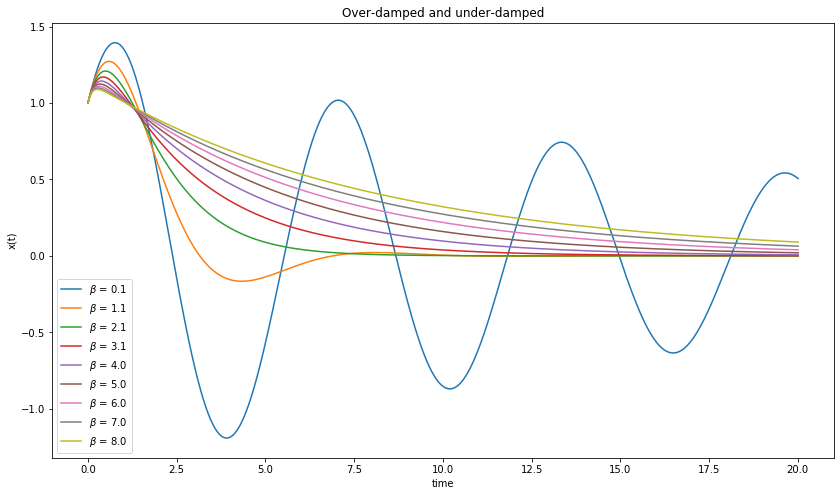
\includegraphics[width=430pt,  height=170pt]{./graphics/q004_a1.png}
										\caption{A plot of $x(t)$  for the under-damped system with varying $\beta$ values} 
										\label{fig:q4a1}
								\end{figure}
								\begin{figure}[!h]
									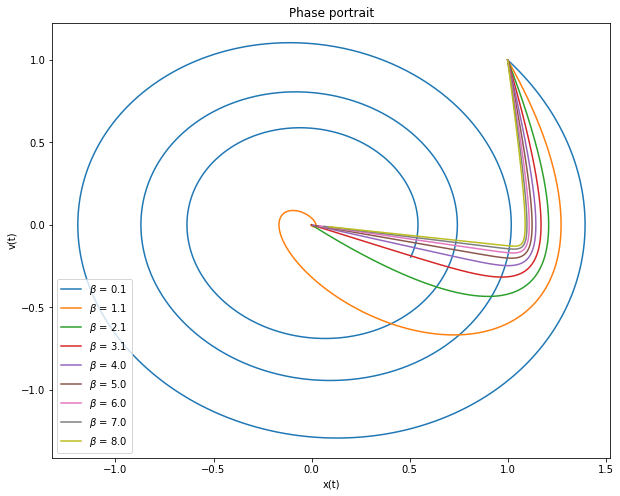
\includegraphics[width=430pt,  height=170pt]{./graphics/q004_a2.png}
										\caption{A plot of the phase portrait  $x(t)$ vs $v(t)$  for the under-damped and over-damped systems with varying $\beta$ values} 
										\label{fig:q4a2}
								\end{figure}
			\item[(b)] When we  switch to a friction force that is more realistic under many circumstances, replacing $\beta x$  with $- \beta \sin \dot{x}$.  The case of the initial condition $ \dot{x}  = 0$,  the friction force is directed against the returning force $x$ and it is equal in magnitude to min$(|x| , \beta )$.  
			\begin{enumerate}
					\item[(i)] A Plot $x(t)$  $ \text{under-damped  and over-damped systems where } 0 < \beta \le 8 $ and the phase diagram for the different $\beta$.
								\begin{figure}[!ht]
									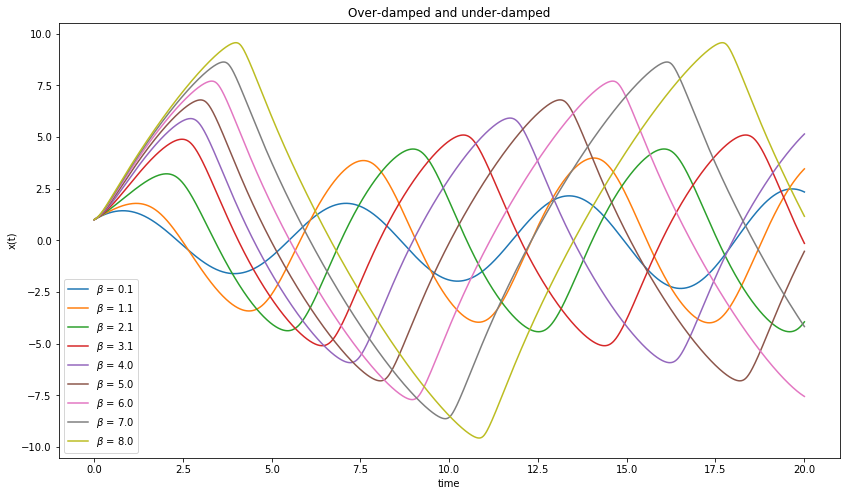
\includegraphics[width=430pt,  height=220pt]{./graphics/q004_b1.png}
										\caption{A plot of $x(t)$  with varying $\beta$ values} 
										\label{fig:q4b1}
								\end{figure}
					\item[(ii)] A plot of the phase diagram for different values of $\beta$.  
							   \begin{figure}[H]
									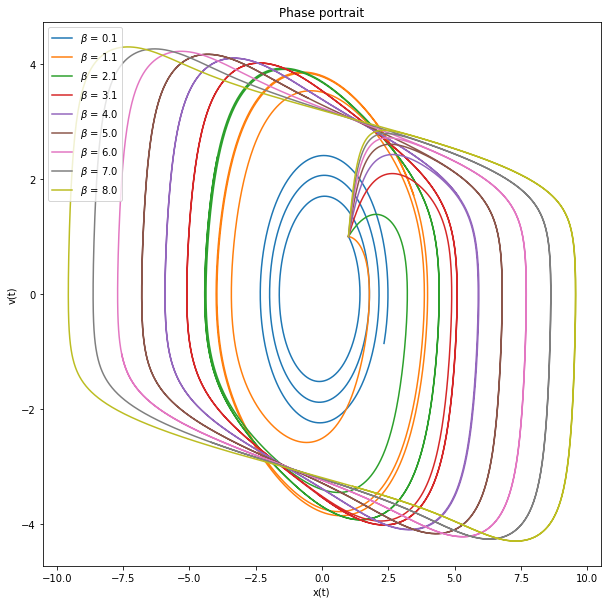
\includegraphics[width=430pt,  height=220pt]{./graphics/q004_b2.png}
										\caption{A plot of the phase portrait  $x(t)$ vs $v(t)$   with varying $\beta$ values} 
										\label{fig:q4b2}
								\end{figure}
			\end{enumerate} 
\end{enumerate}
\end{document}